\section{Statistical Models}
\label{ch:statmodel}

Primary source for this was Hyndman-et-al-2018 %\cite{Hyndman-et-al-2018}.

\subsection{Holt-Winters’ seasonal method}

\begin{figure}
\begin{tcolorbox}[width=.6\textwidth]%

Suppose there are $N$ observations.

Initial step:

$\left|\begin{array}{l}
L_s = \frac1s \sum_{i=1}^s y_i \\
b_s = \frac1s \left[\frac{y_{s+1}-y_1}{s}+\frac{y_{s+2}-y_2}{s}+\dots+\frac{y_{2s}-y_s}{s}\right]\\
S_i  = \frac{y_i}{L_s}, \ i=1,\dots,s
\end{array}\right.$

and choose parameters $0\leq\alpha\leq1,\ 0\leq\beta\leq1$ and $0\leq\gamma\leq1$

Then compute for $s<t\leq N$:

$\left|\begin{array}{lll}
\text{Level} &       L_t & = \alpha \frac{y_t}{S_{t-s}}+(1-\alpha)(L_{t-1}+b_{t-1})\\
\text{Trend} &      b_t & = \beta(L_t-L_{t-1})+(1-\beta)b_{t-1}\\
\text{Seasonal} & S_t & = \gamma \frac{y_t}{L_t} + (1-\gamma)S_{t-s}\\
\text{Forecast} & F_{t+1} & = (T_t+b_t)S_{t+1-s}
\end{array}\right.$

For subsequent observations, 

$F_{N+k}=(L_N+k\cdot b_N) S_{N+k-s}$

\label{SHWx}
\end{tcolorbox}
\caption{Seasonal Holt Winter’s Multiplicative Model Algorithm (denoted SHW$_\times$)}
\end{figure}

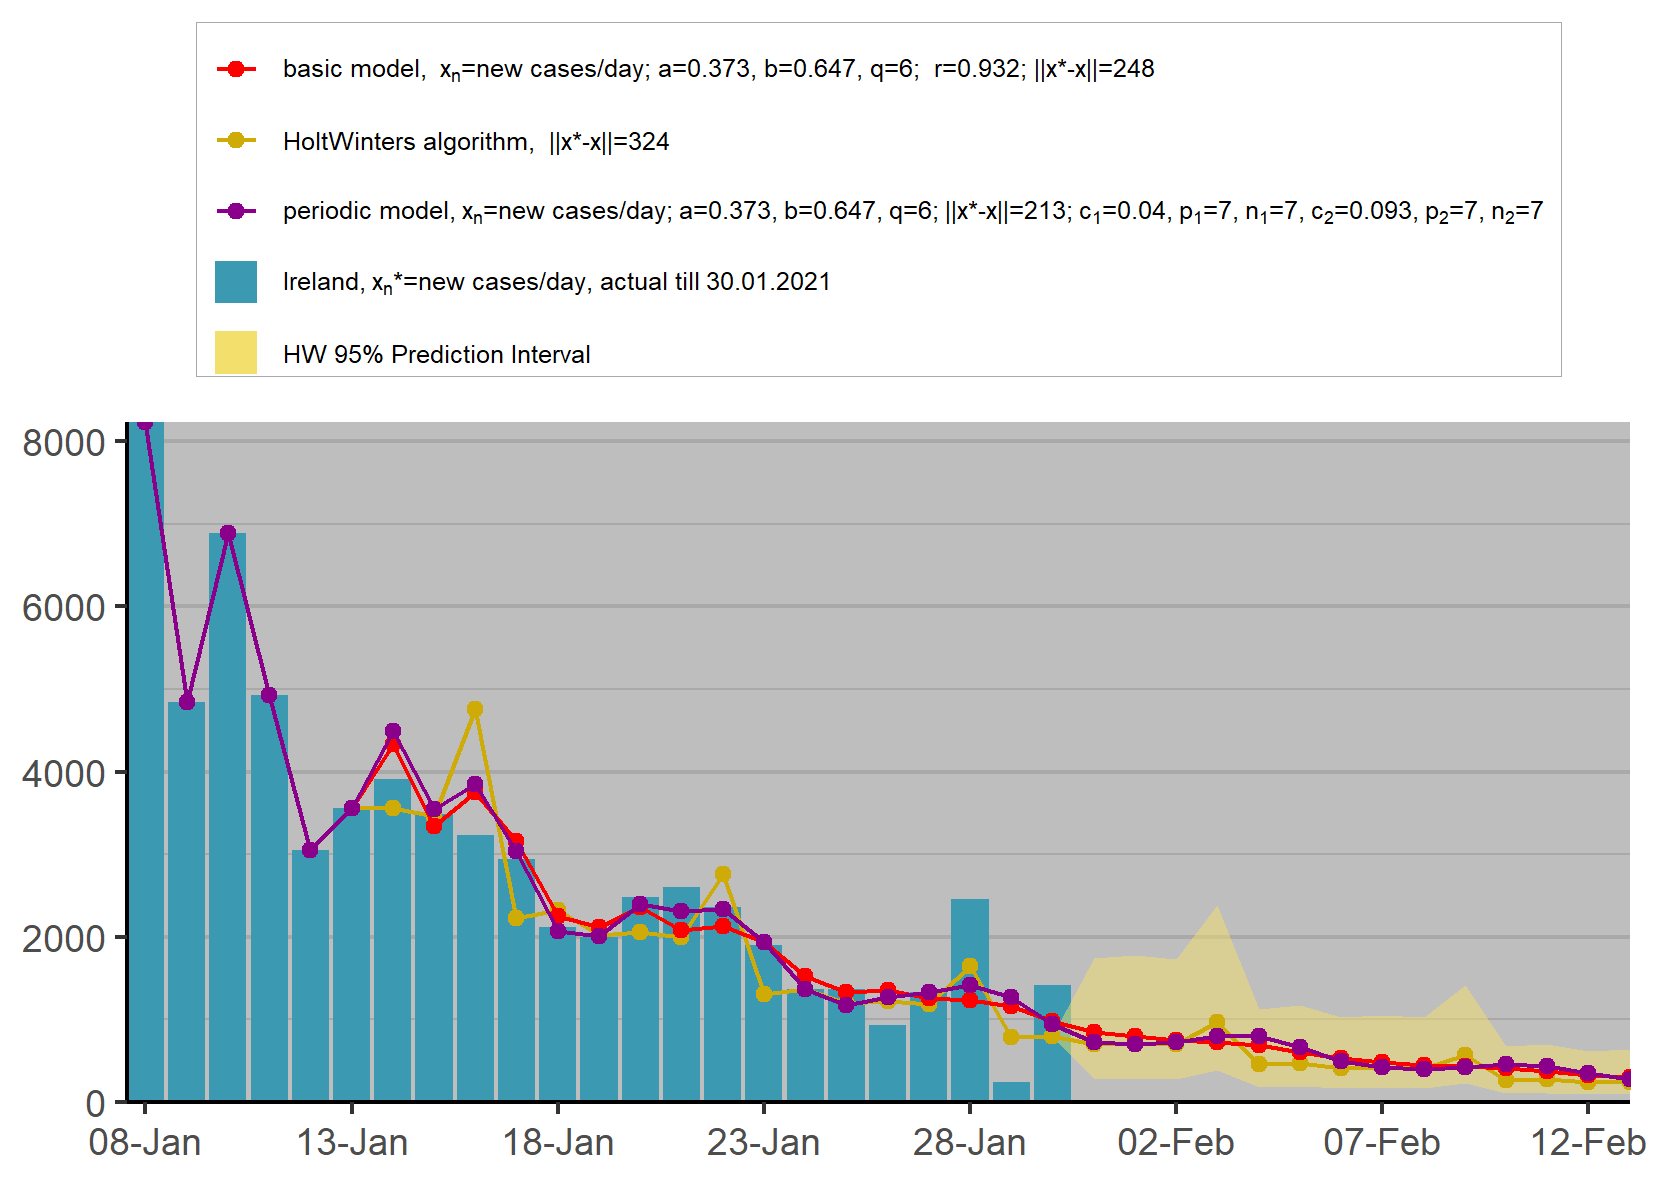
\includegraphics[width=0.9\textwidth]{Ireland-hw.png}

\begin{figure}[!htb]
\minipage{0.48\textwidth}
  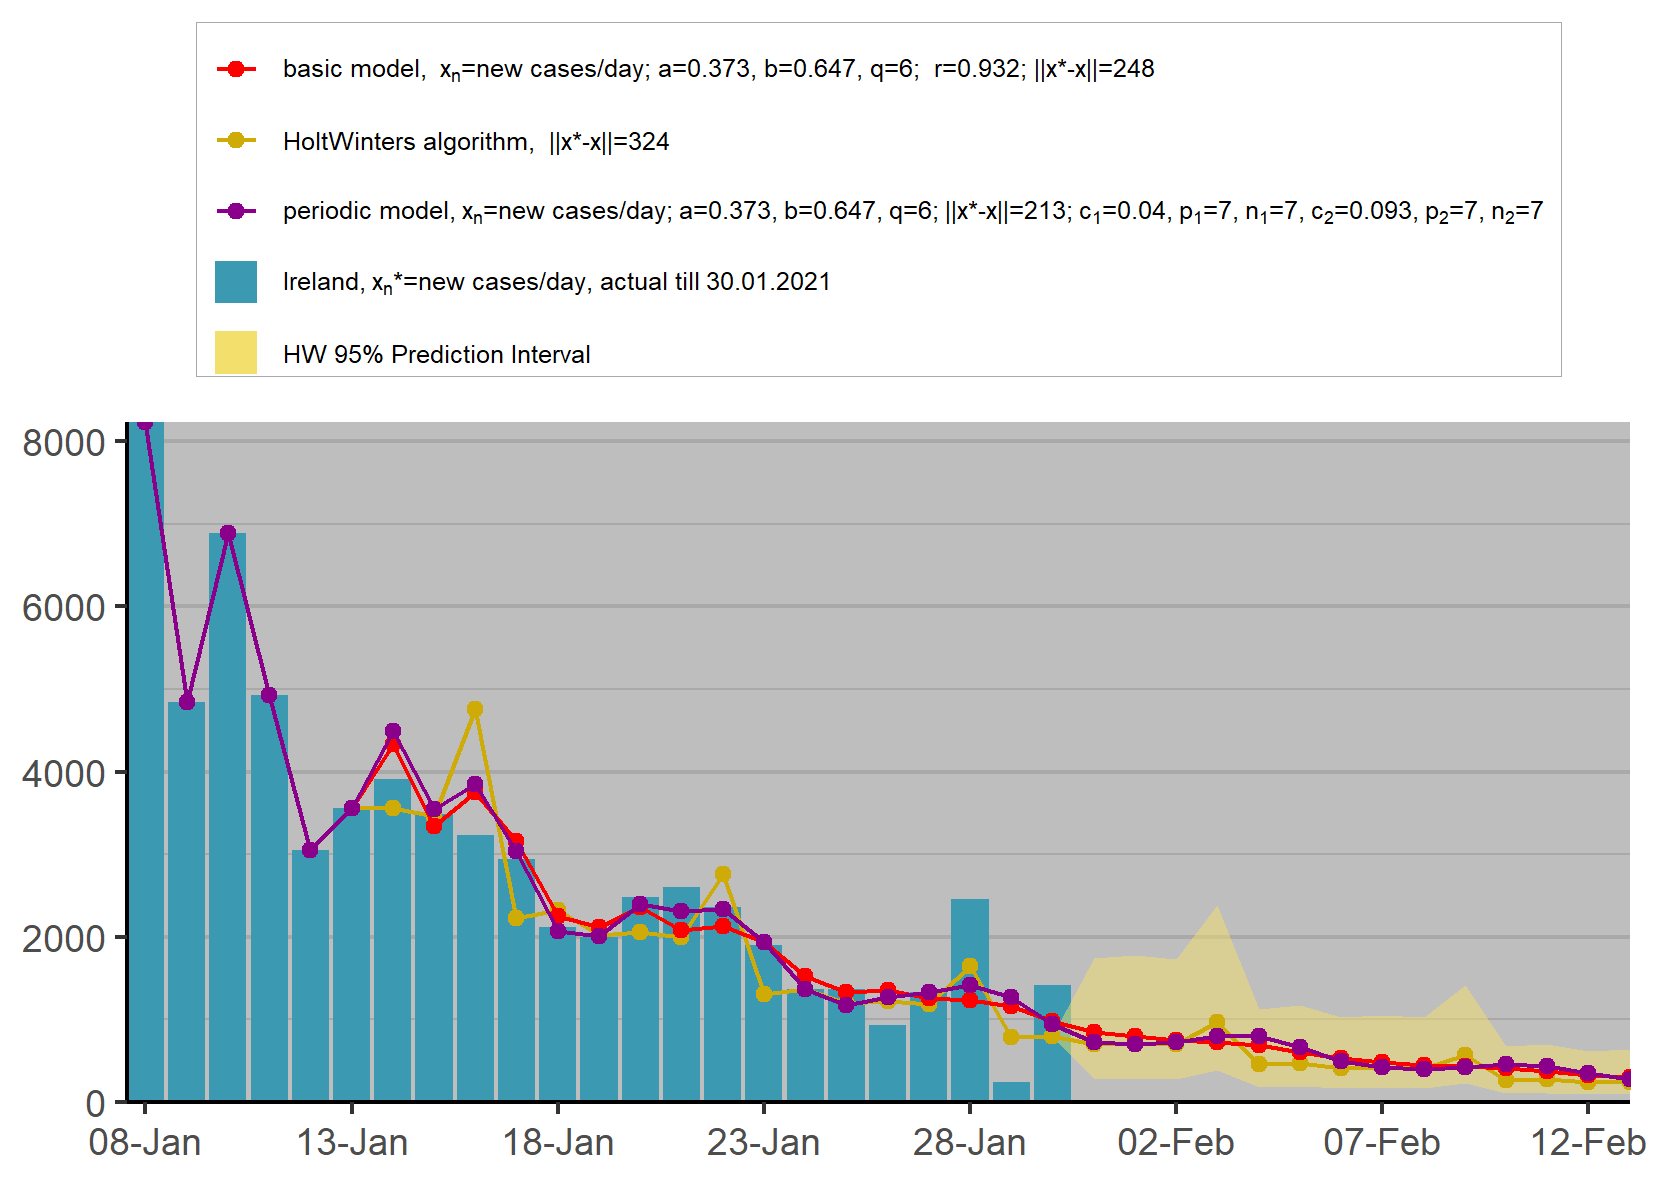
\includegraphics[width=\linewidth]{Ireland-hw.png} \label{fig:ireland-hw}
\endminipage\hfill
\minipage{0.48\textwidth}
  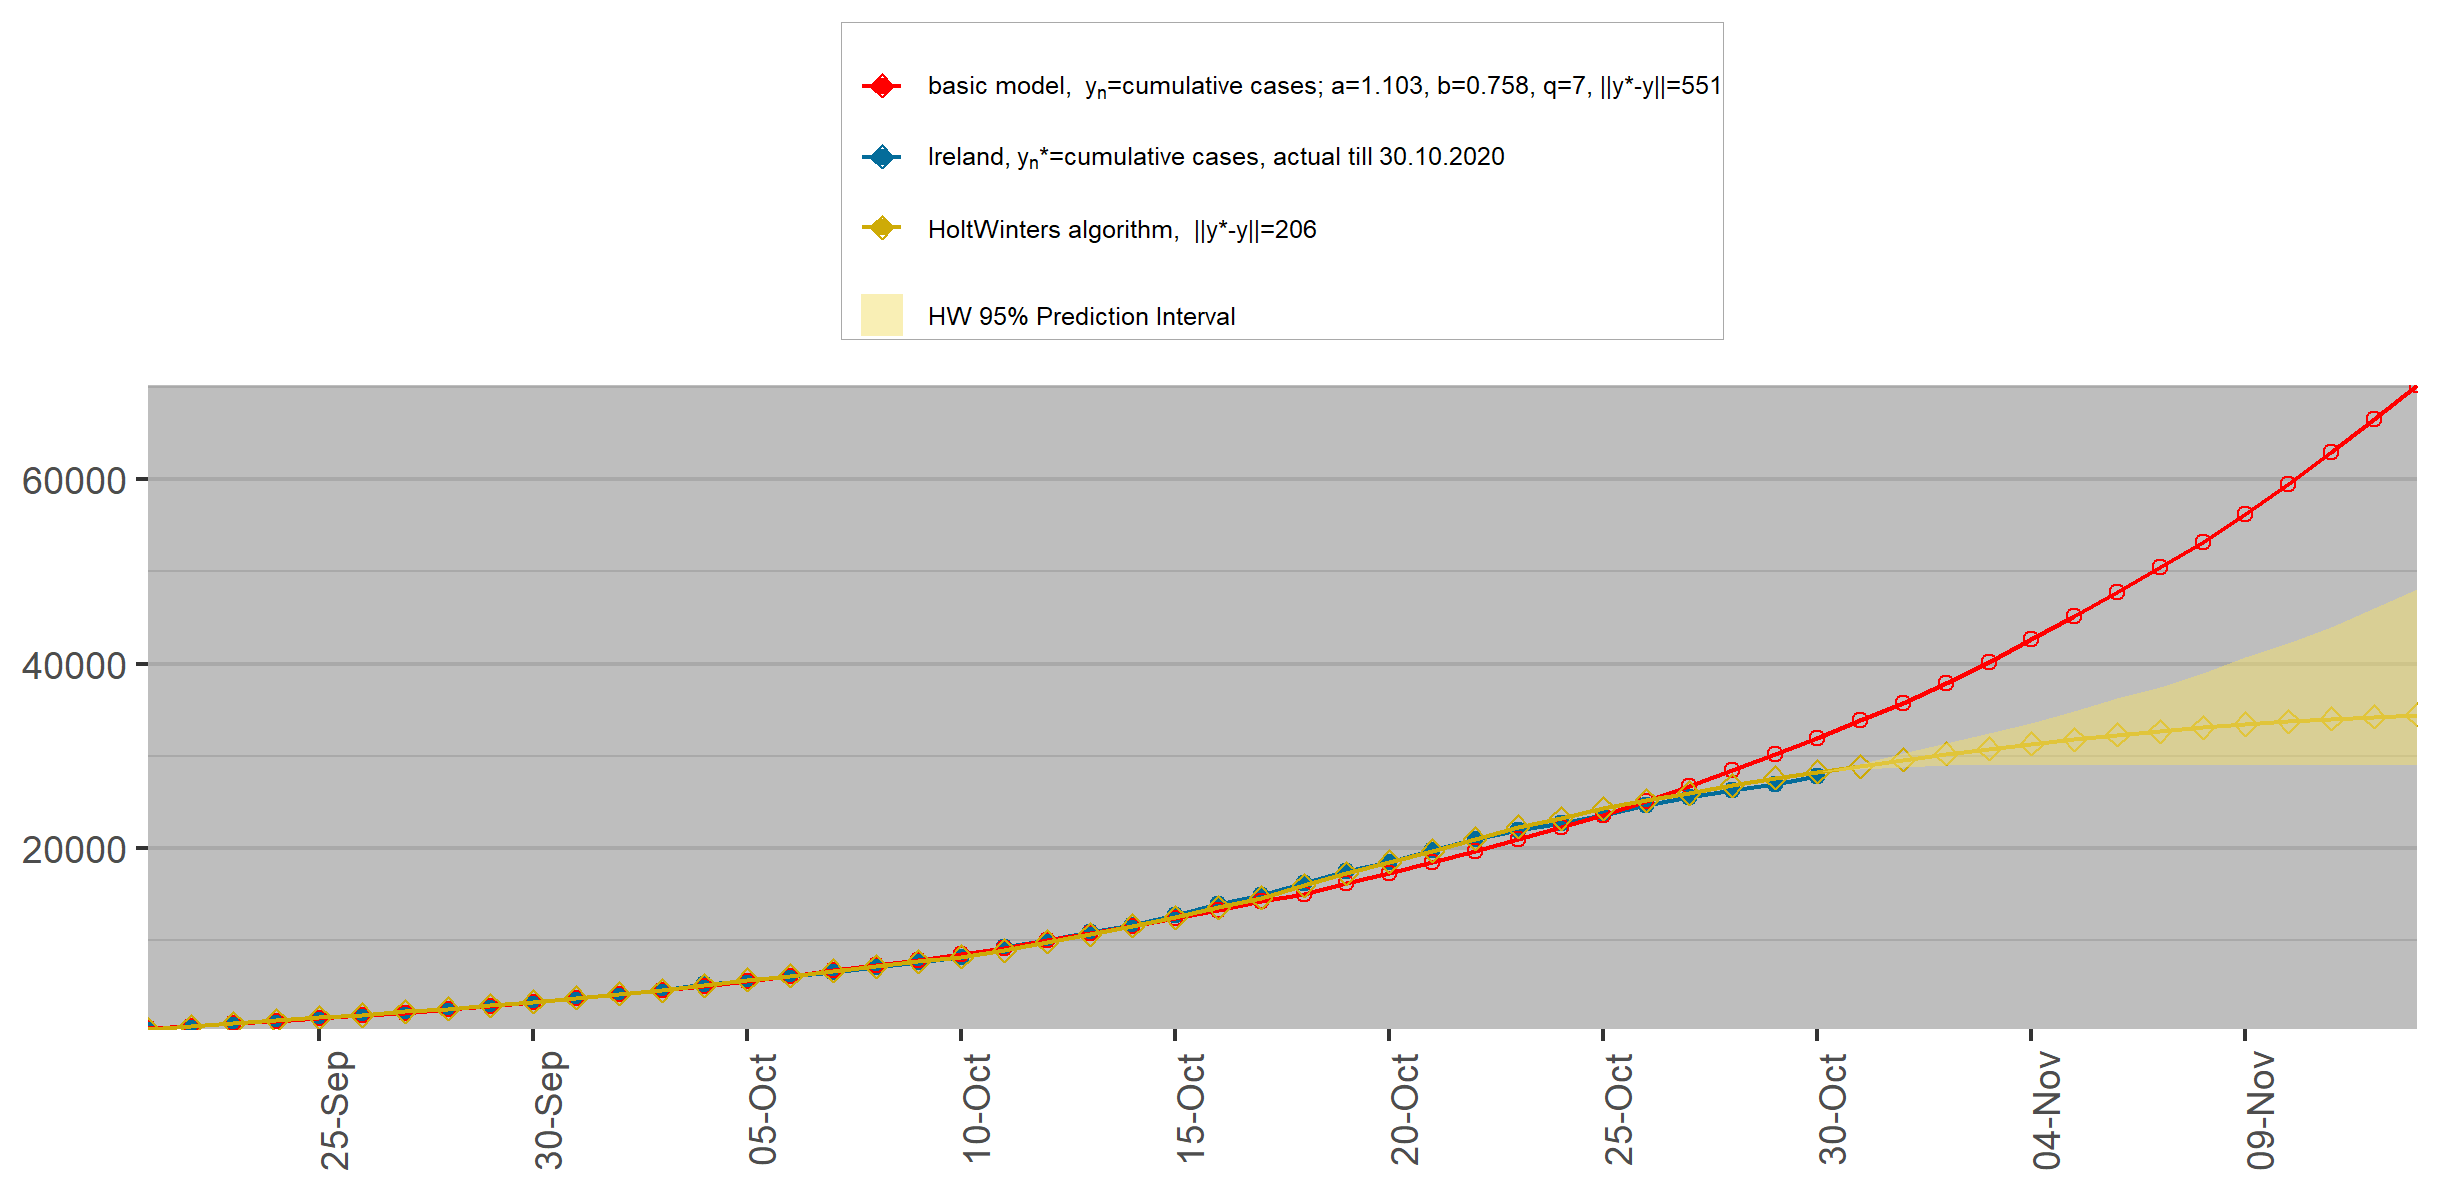
\includegraphics[width=\linewidth]{Ireland-hwy.png} \label{fig:ireland-hwy}
\endminipage
\caption{HoldWinters model, Ireland}
\end{figure}


\subsection{ARIMA models}

\begin{figure}[!htb]
\minipage{0.48\textwidth}
  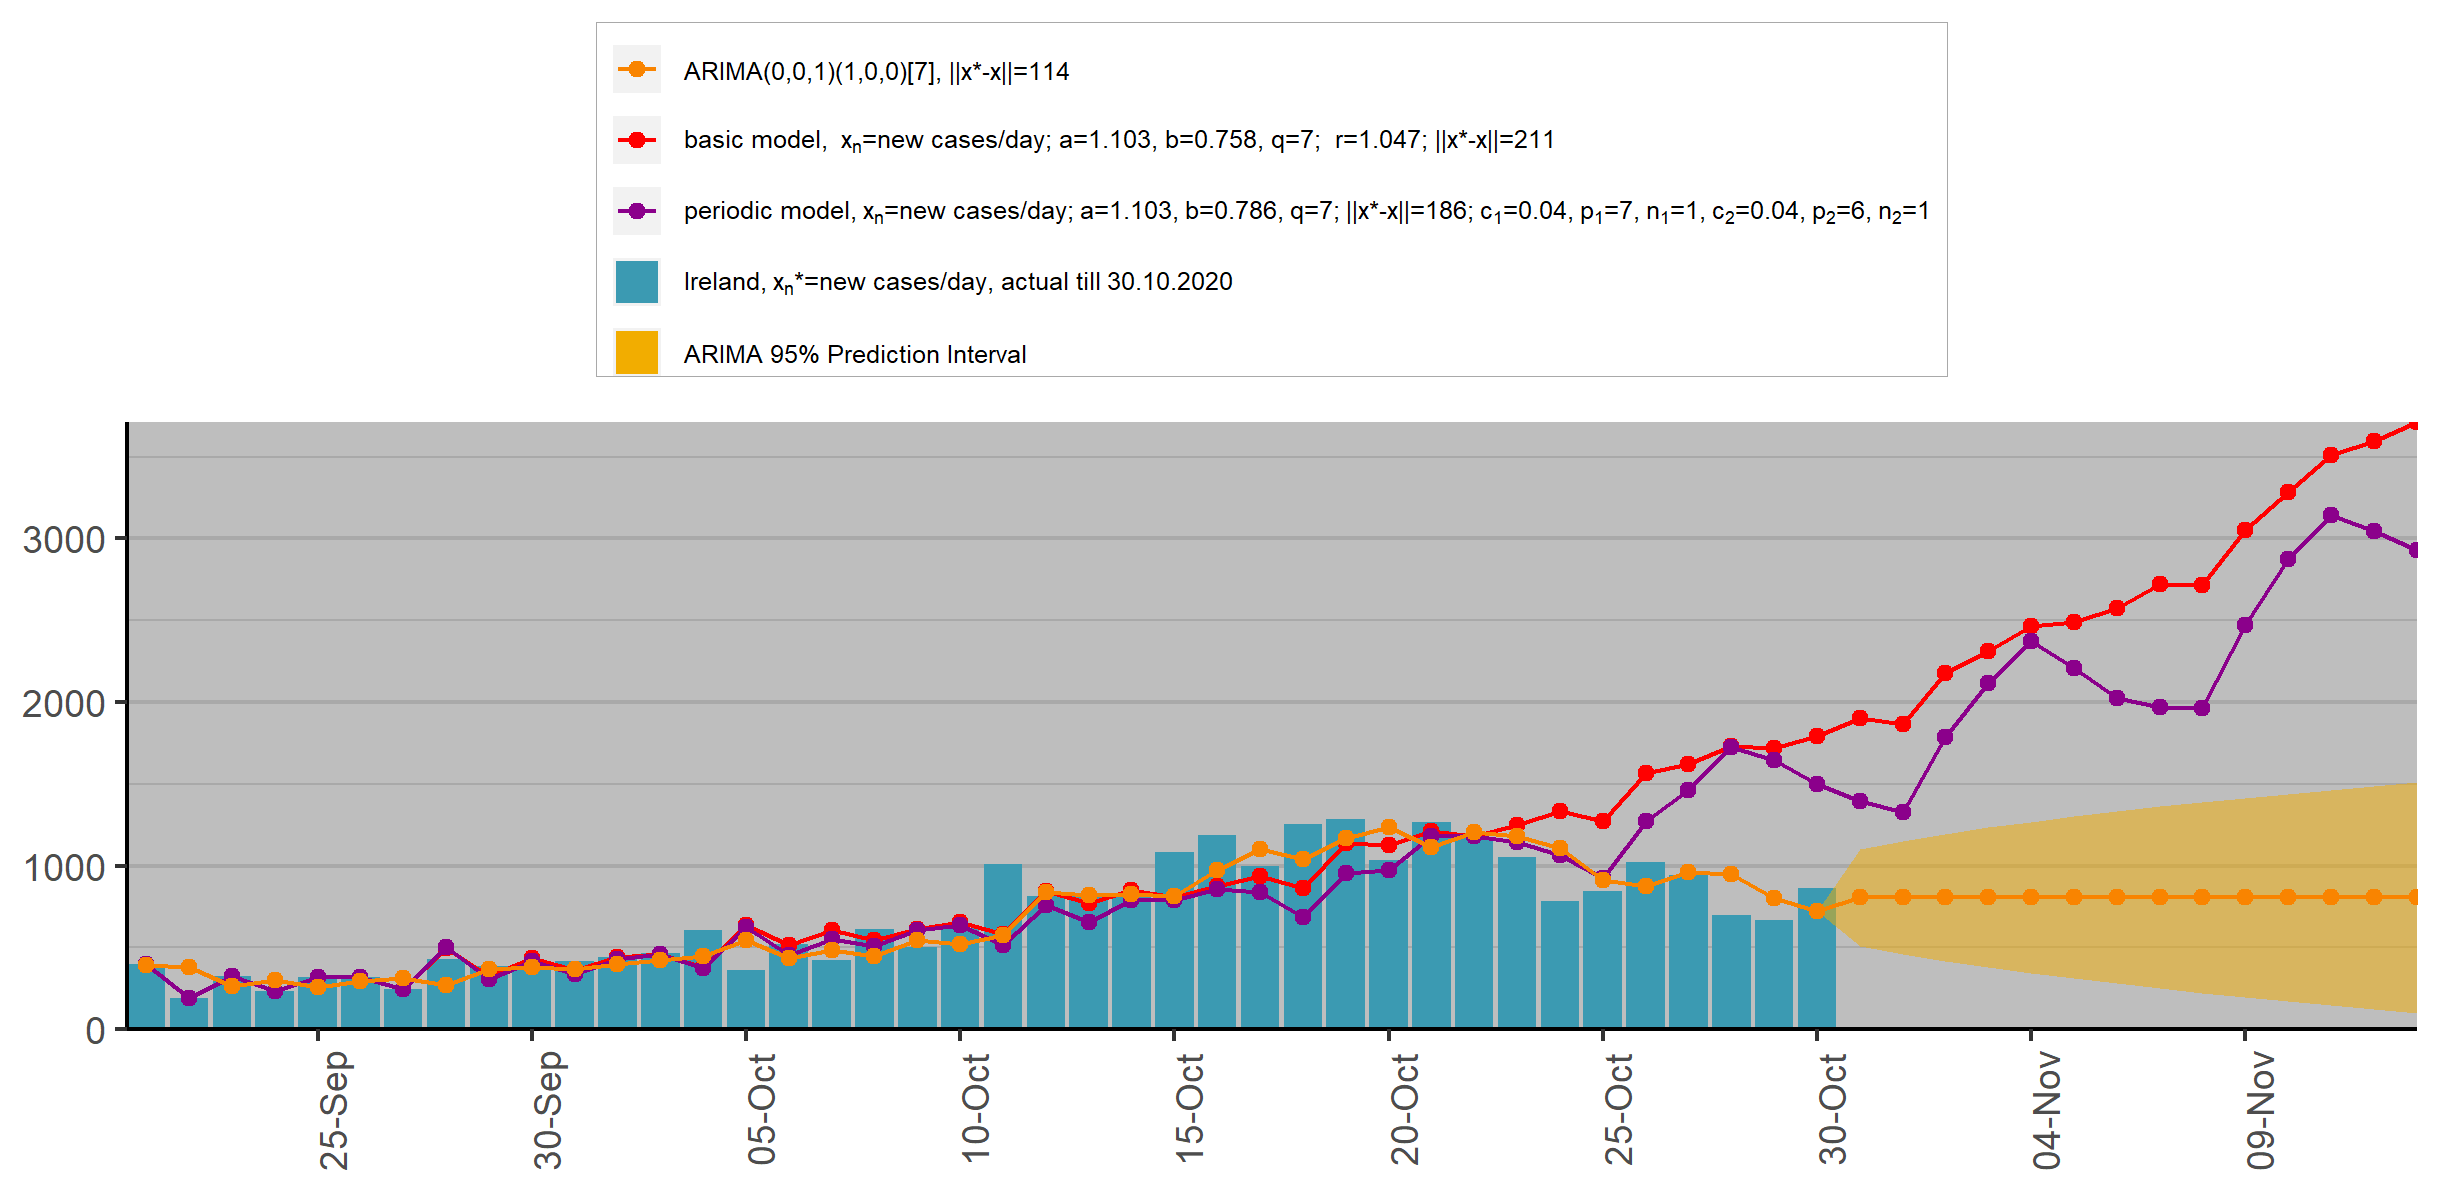
\includegraphics[width=\linewidth]{Ireland-arima.png} \label{fig:ireland-arima}
\endminipage\hfill
\minipage{0.48\textwidth}
  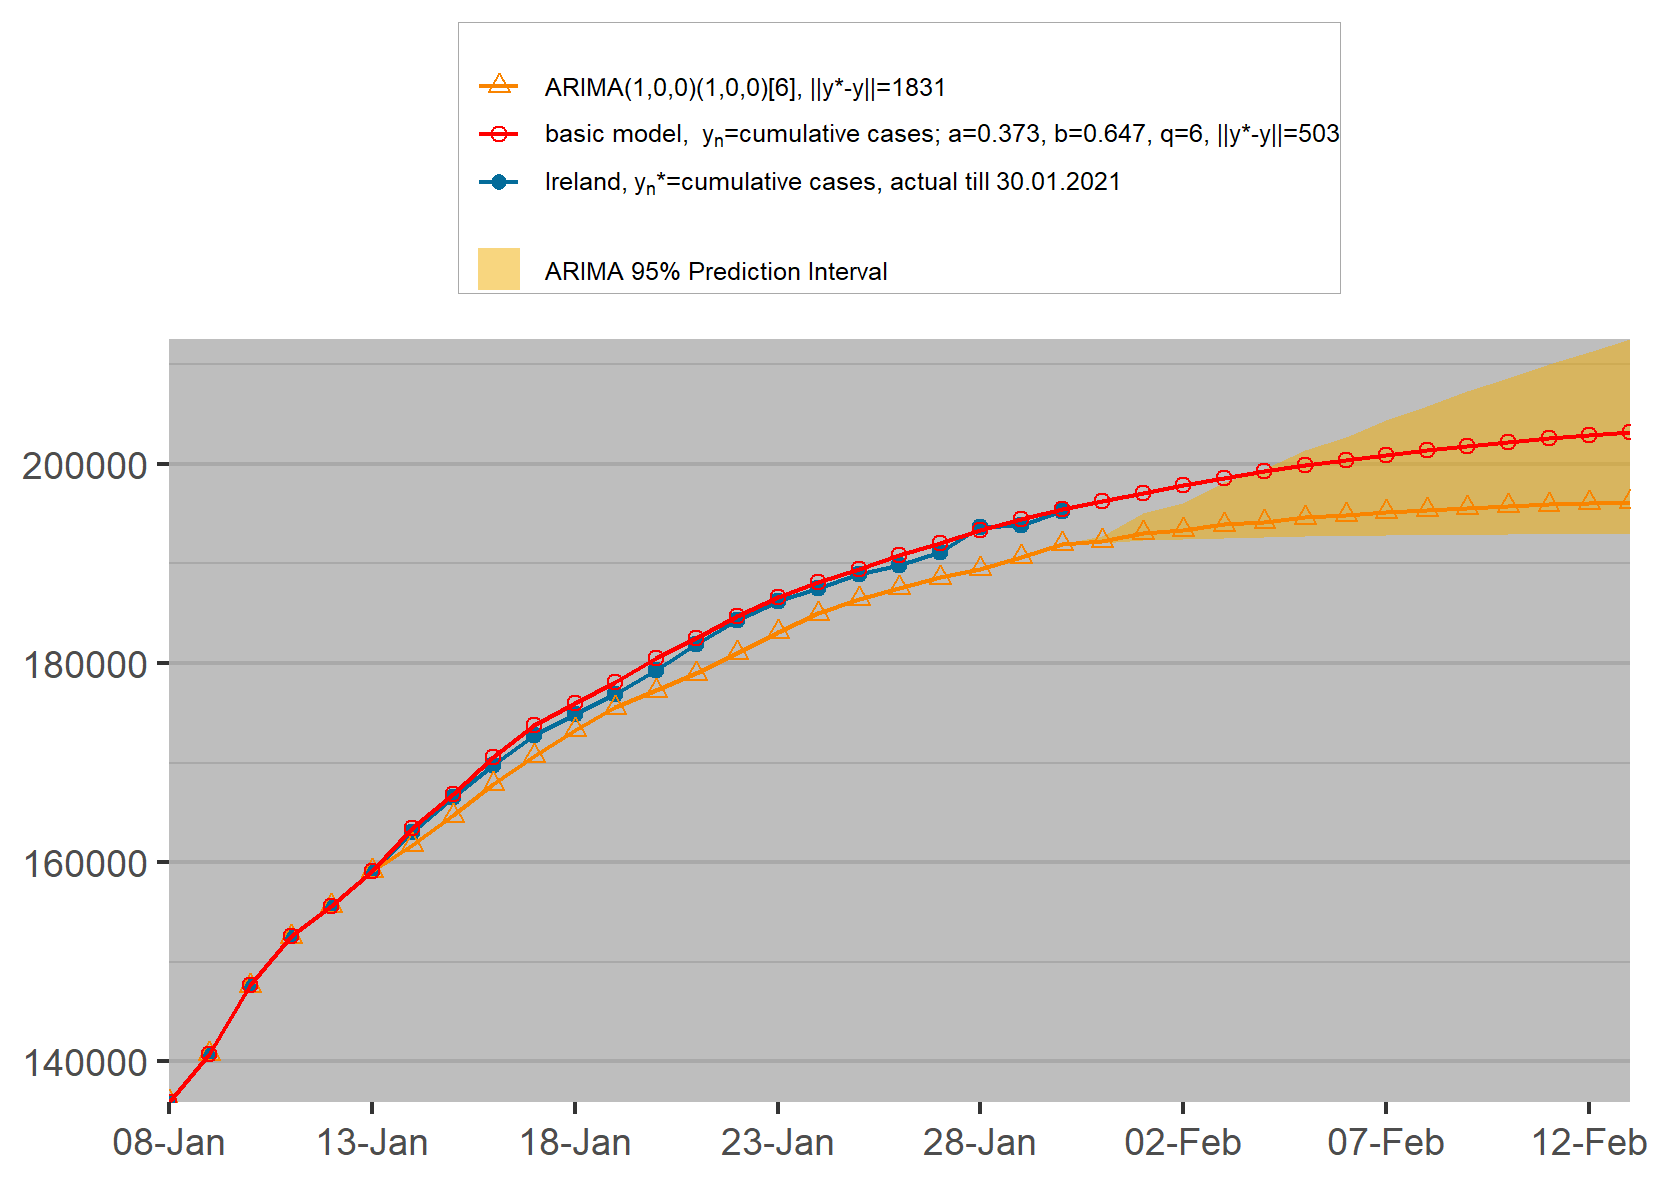
\includegraphics[width=\linewidth]{Ireland-arimay.png} \label{fig:ireland-arimay}
\endminipage
\caption{ARIMA model, Ireland}
\end{figure}

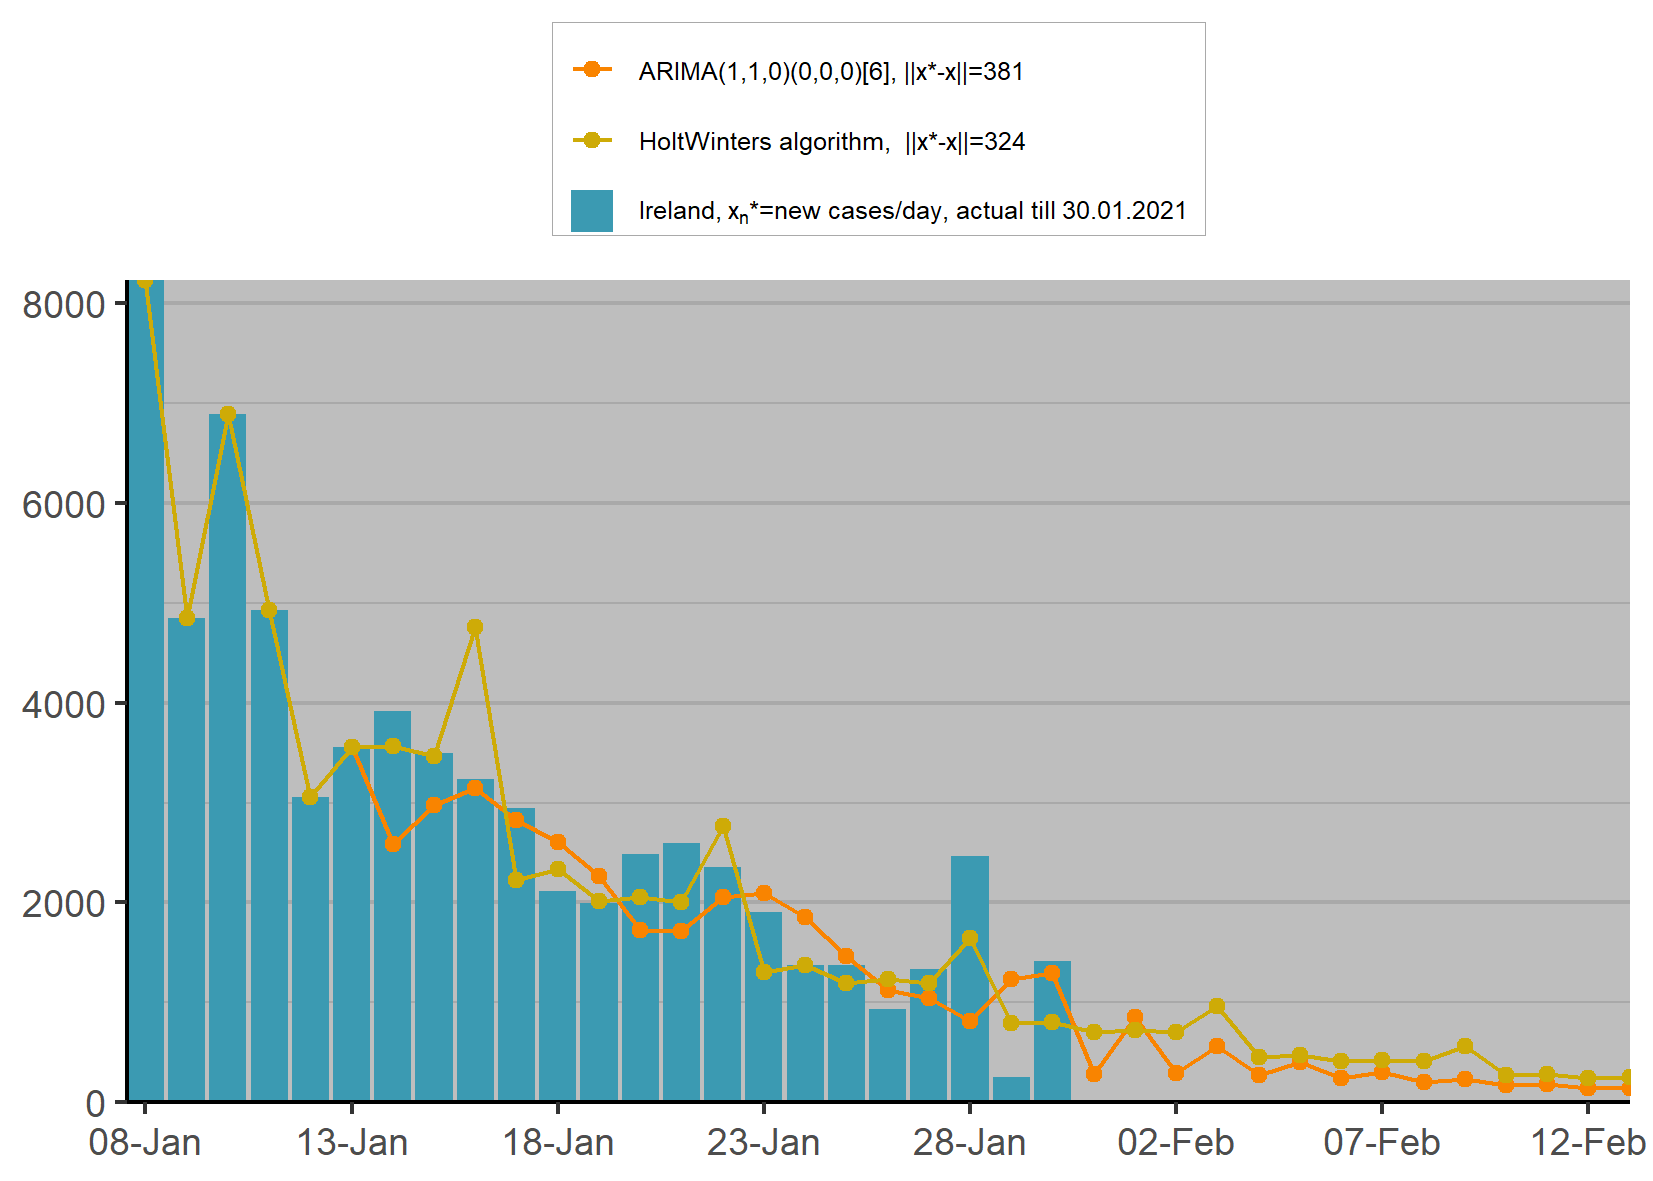
\includegraphics[width=0.9\textwidth]{Ireland-hwarima.png}


\subsection{Neural network models}

\begin{figure}[!htb]
\minipage{0.48\textwidth}
  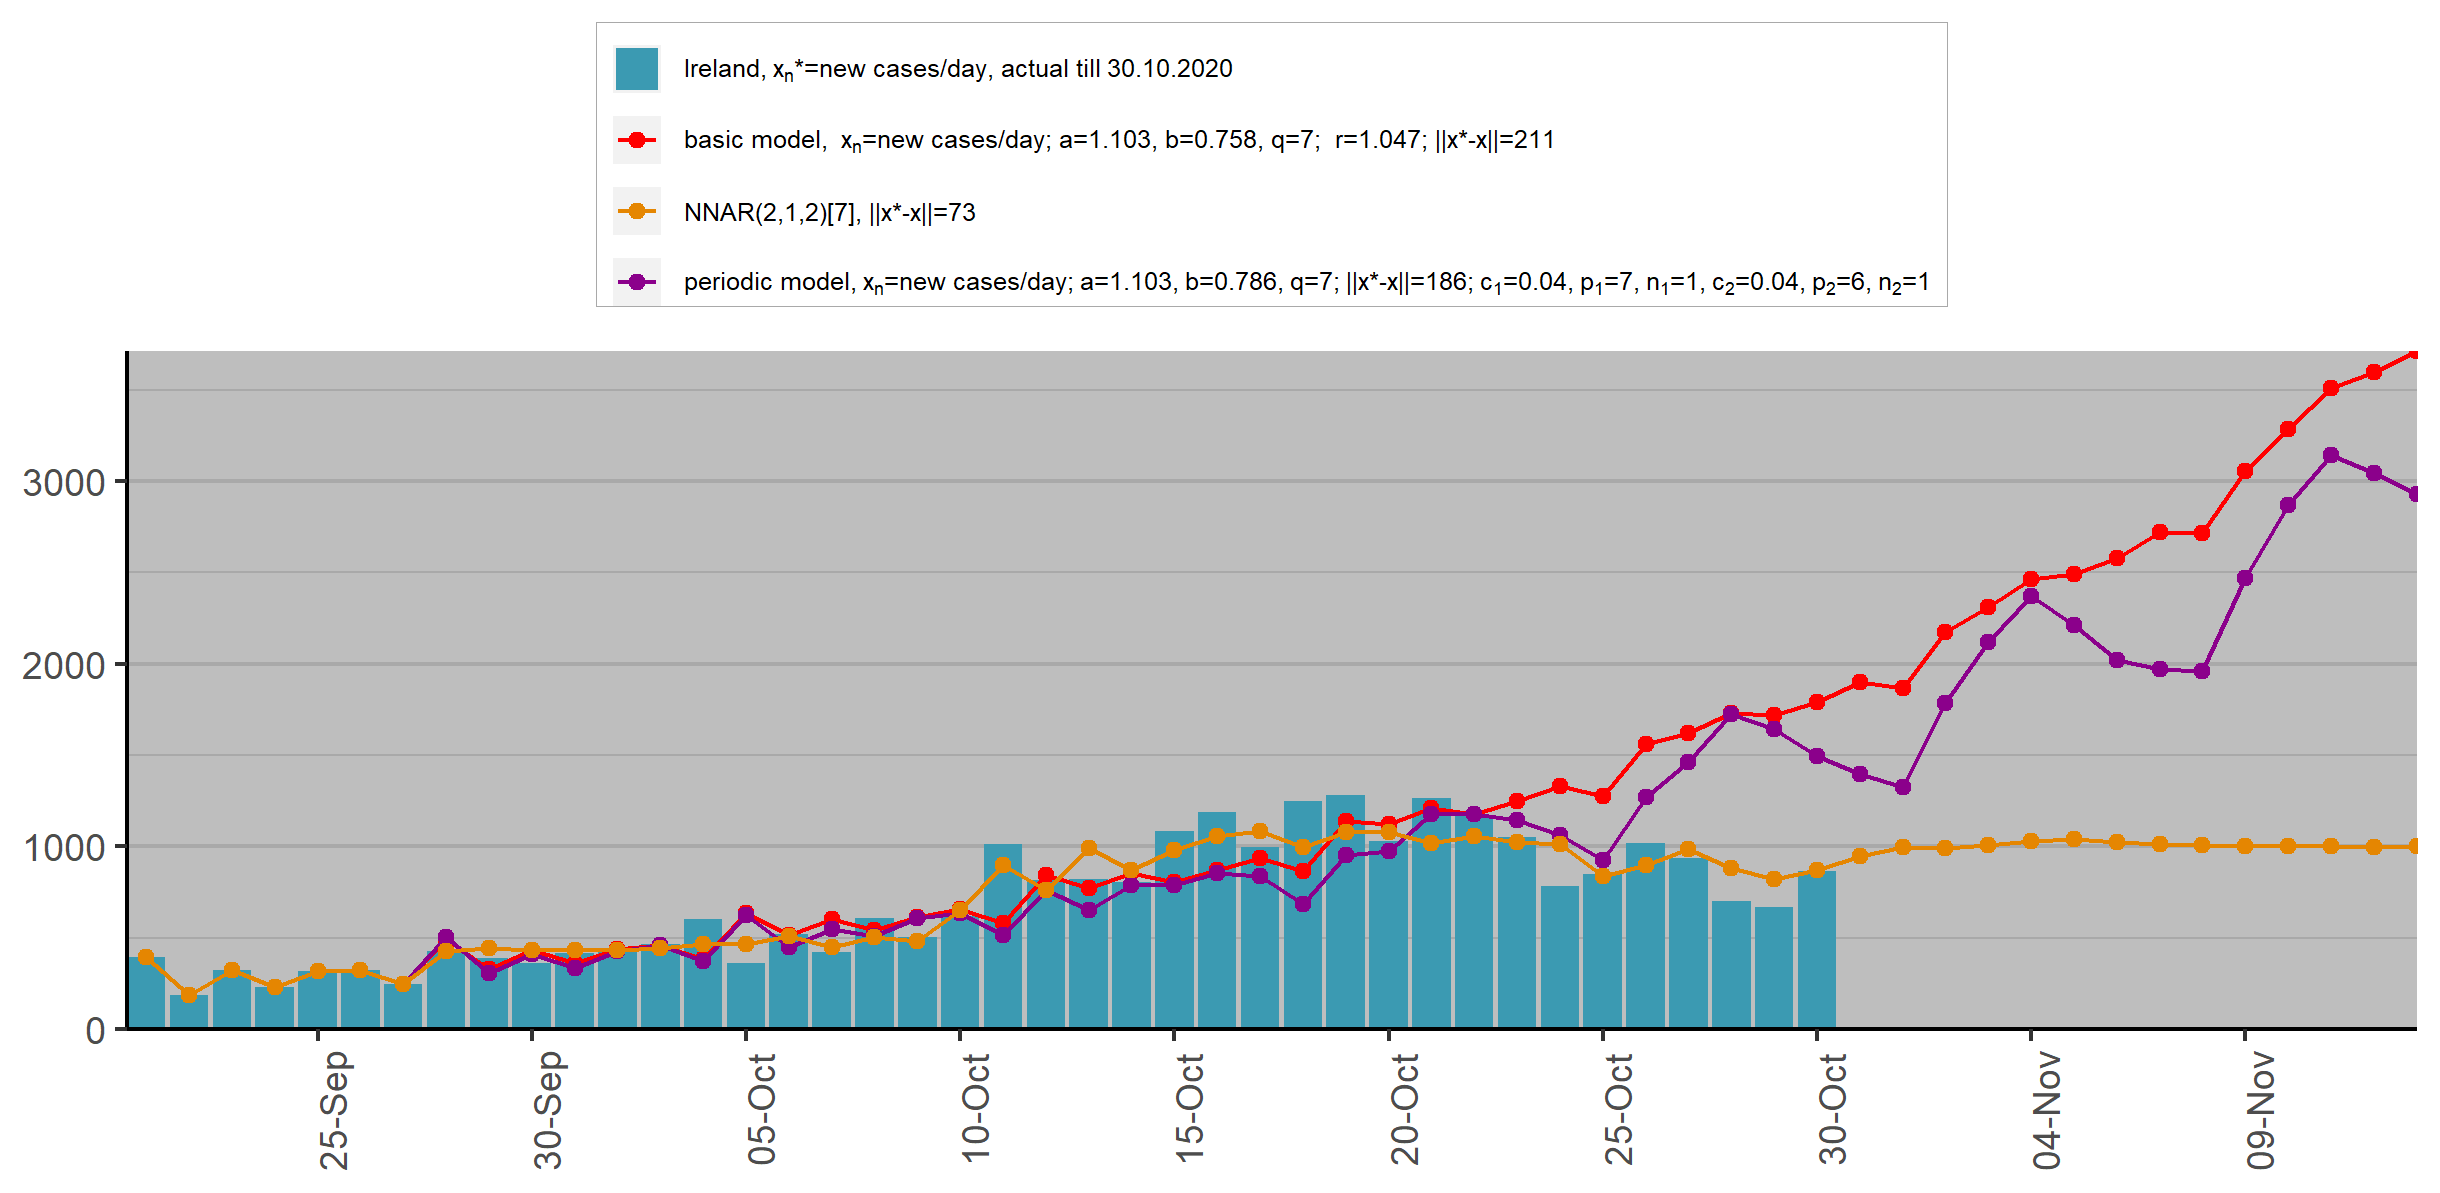
\includegraphics[width=\linewidth]{Ireland-nn.png} \label{fig:ireland-nn}
\endminipage\hfill
\minipage{0.48\textwidth}
  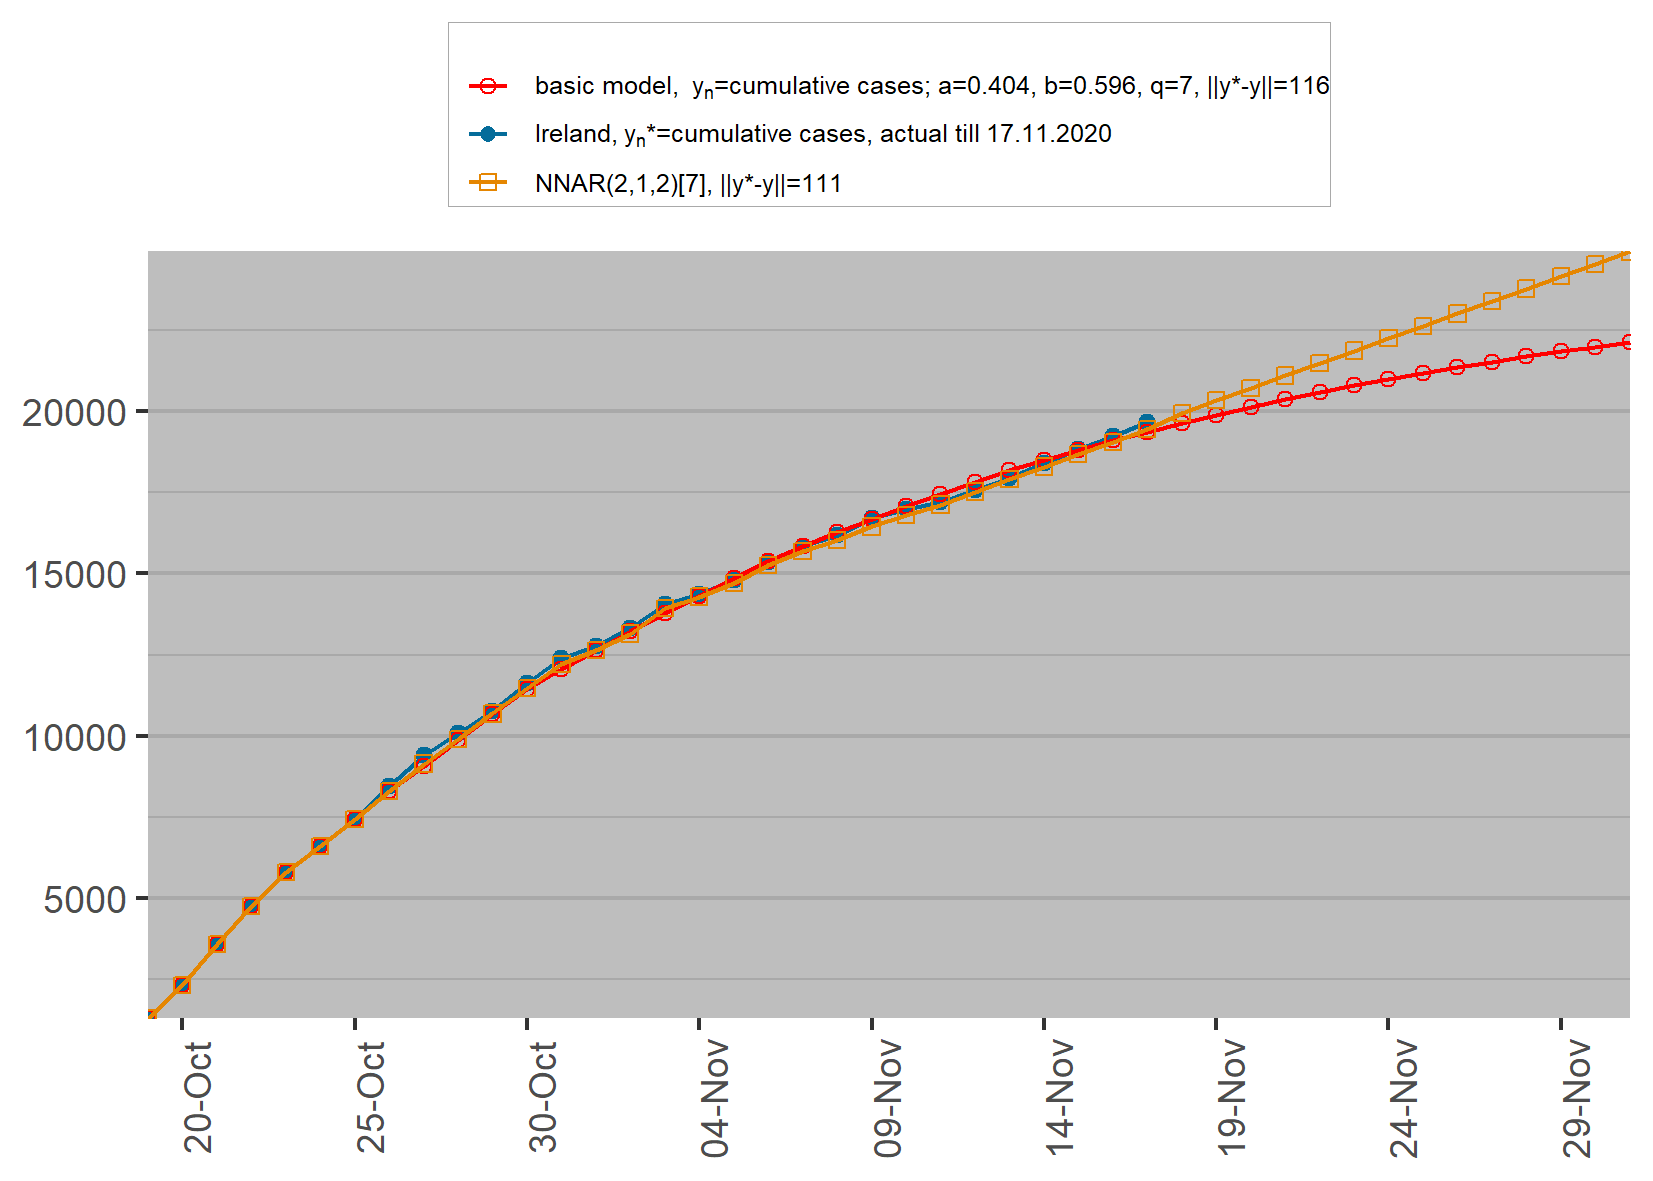
\includegraphics[width=\linewidth]{Ireland-nny.png} \label{fig:ireland-nny}
\endminipage
\caption{Neural Network model, Ireland}
\end{figure}
